\section{Шифратор}

Шифратор (или кодер, CD) (англ. \emph{encoder}) -- это логическое устройство,
выполняющее логическую операцию преобразования позиционного \( n \)-разрядного
кода в \( m \)-разрядный двоичный код.

При подаче сигнала на один из \( n \) входов (обязательно на один, не более) на
выходе появляется двоичный код номера активного входа.

Если количество входов настолько велико, что в шифраторе используются все
возможные комбинации сигналов на выходе, то такой шифратор называется полным,
если не все, то неполным.

Число входов и выходов в полном шифраторе связано соотношением:\\
\( n = 2^m \), где \( n \) -- число входов, \( m \) -- число выходных двоичных
разрядов. В неполном шифраторе число \( m \) обычно выбирается минимально
возможным для операции шифрования, например, для \( n = 10 \) число двоичных
разрядов \( m = 4 \), для \( n = 25 \): \( m = 5 \).

Таким образом, назначение шифратора -- подавать на выход информацию о том, на
какой из входов подан сигнал.
 
Таблица истинности и функциональная схема полного шифратора \( 4\times2 \)
приведены соответственно в таблице \ref{tab_cd} и на рисунке \ref{pic_cd}. На
рисунке \ref{pic_cd_s} приведено условное обозначение шифраторов на схеме на
примере шифратора \( 8\times3 \).
    
\begin{table}[!ht]
    \centering
    \caption{Таблица истинности шифратора \( 4\times2 \)}
    \label{tab_cd}
    \begin{tabular}{|*{6}{C{.12}|}} \hline
        \( A_3 \) & \( A_2 \) & \( A_1 \) & \( A_0 \) & \( x_0 \) &
        \( x_1 \) \\ \hline
        0 & 0 & 0 & 1 & 0 & 0 \\ \hline
        0 & 0 & 1 & 0 & 0 & 1 \\ \hline
        0 & 1 & 0 & 0 & 1 & 0 \\ \hline
        1 & 0 & 0 & 0 & 1 & 1 \\ \hline
    \end{tabular}
\end{table}

\vspace*{1em}
\begin{figure}[!ht]
    \begin{minipage}{.65\textwidth}
        \centering
        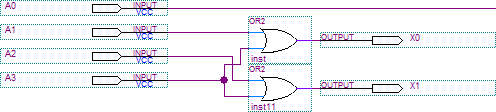
\includegraphics[width=\textwidth]{coder}
        \caption{Схема шифратора \( 4\times2 \)}
        \label{pic_cd}
    \end{minipage}
    \hfill
    \begin{minipage}{.3\textwidth}
        \centering
        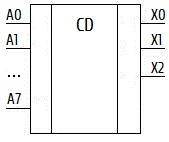
\includegraphics{cd}
        \caption{Обозначение шифраторов на схемах}
        \label{pic_cd_s}
    \end{minipage}
\end{figure}

\newpage % --------------------------------------------------------------------
\section{Дешифратор}
Дешифратор (или декодер, DC) (англ. \emph{decoder}) -- это логическое
устройство, преобразующее \( n \)-разрядный двоичный код в \( m \)-ичный
одноединичный код, где \( m \) -- количество выходов устройства.
Логический сигнал появляется на том выходе, порядковый номер которого
соответствует двоичному коду.

Двоичный дешифратор работает по следующему принципу: пусть дешифратор имеет
\( n \) входов, на них подан двоичный код, тогда на выходе будем иметь такой
код, разрядности меньшей или равной \( m = 2^n \), что разряд, номер которого
равен входному слову, принимает значение единицы, все остальные разряды равны
нулю.

Очевидно, что максимально возможная разрядность выходного кода равна \( m \).
Такой дешифратор называется полным. Если часть входных наборов не используется,
то число выходов меньше \( m \), и дешифратор является неполным.

Таким образом, назначение дешифратора -- подавать на один из выходов логическую
единицу в зависимости от информации на входе.

Таблица истинности и функциональная схема полного дешифратора \( 2\times4 \)
приведены соответственно в таблице \ref{tab_dc} и на рисунке \ref{pic_dc}. На
рисунке \ref{pic_dc_s} приведено условное обозначение дешифраторов на схеме на
примере дешифратора \( 3\times8 \).
    
\begin{table}[!ht]
    \centering
    \caption{Таблица истинности дешифратора \( 2\times4 \)}
    \label{tab_dc}
    \begin{tabular}{|*{6}{C{.12}|}} \hline
        \( A_1 \) & \( A_0 \) & \( D_3 \) & \( D_2 \) & \( D_1 \) & \( D_0 \)
        \\ \hline
        0 & 0 & 0 & 0 & 0 & 1 \\ \hline
        0 & 1 & 0 & 0 & 1 & 0 \\ \hline
        1 & 0 & 0 & 1 & 0 & 0 \\ \hline
        1 & 1 & 1 & 0 & 0 & 0 \\ \hline
    \end{tabular}
\end{table}

\begin{figure}[!ht]
    \begin{minipage}{.65\textwidth}
        \centering
        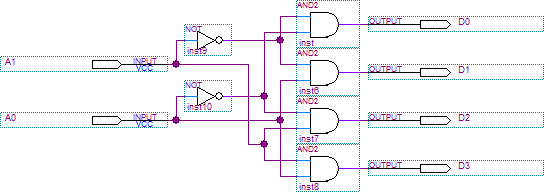
\includegraphics[width=\textwidth]{decoder}
        \caption{Схема дешифратора \( 2\times4 \)}
        \label{pic_dc}
    \end{minipage}
    \hfill
    \begin{minipage}{.3\textwidth}
        \centering
        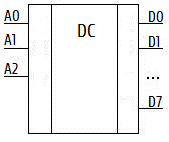
\includegraphics{dc}
        \caption{Обозначение дешифраторов на схемах}
        \label{pic_dc_s}
    \end{minipage}
\end{figure}

\newpage % --------------------------------------------------------------------
\section{Мультиплексор}

Мультиплексор (MUX) (англ. \emph{multiplexer}) -- это логическое устройство,
коммутирующее один из своих входов с единственным выходом в зависимости от
управляющего сигнала.

Если количество управляющих (или адресных) входов \( n \), то максимально
возможное количество информационных входов \( m = 2^n \). Функционально
мультиплексор состоит из \( m \) элементов конъюнкции, выходы которых объединены дизъюнктивно с \( m \)
входами. На одни входы всех элементов конъюнкции подаются информационные
сигналы, а другие входы этих элементов соединены с соответствующими выходами
дешифратора с \( n \) входами.

Таким образом, назначение мультиплексора -- подавать на выход сигнал с одного
из информационных входов в зависимости от кода на управляющих входах.

Таблица истинности и функциональная схема двухбитного мультиплексора приведены
соответственно в таблице \ref{tab_mux} и на рисунке \ref{pic_mux}. На
рисунке \ref{pic_mux_s} приведено условное обозначение мультиплексоров на схеме
на примере того же двухбитного мультиплексора.

\begin{table}[!ht]
    \centering
    \caption{Таблица истинности двухбитного мультиплексора}
    \label{tab_mux}
    \begin{tabular}{|*{3}{C{.12}|}} \hline
        \( D_1 \) & \( D_0 \) & \( C \) \\ \hline
        0 & 0 & \( A_0 \) \\ \hline
        0 & 1 & \( A_1 \) \\ \hline
        1 & 0 & \( A_2 \) \\ \hline
        1 & 1 & \( A_3 \) \\ \hline
    \end{tabular}
\end{table}
\vspace*{-1em}
\begin{figure}[!ht]
    \begin{minipage}{.7\textwidth}
        \centering
        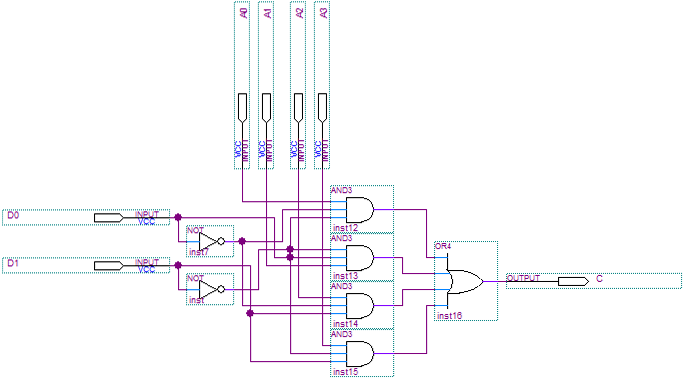
\includegraphics[width=\textwidth]{multiplexer}
        \caption{Схема двухбитного мультиплексора}
        \label{pic_mux}
    \end{minipage}
    \hfill
    \begin{minipage}{.25\textwidth}
        \centering
        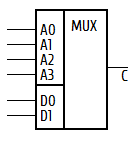
\includegraphics{mux}
        \caption{Обозначение мультиплексоров на схемах}
        \label{pic_mux_s}
    \end{minipage}
\end{figure}

\newpage % --------------------------------------------------------------------
\section{Демультиплексор}

Демультиплексор (DMX) (англ. \emph{demultiplexer}) -- это логическое
устройство, обеспечивающее соединение одного из своих информационных выходов с
одним входом в зависимости от управляющего сигнала.

Если количество адресных входов \( n \), то максимально возможное количество
информационных выходов \( m = 2^n \). Функционально демультиплексор состоит из
\( m \) элементов конъюнкции. На одни входы всех элементов конъюнкции подается
информационный сигнал, а другие входы этих элементов соединены с
соответствующими выходами дешифратора с \( n \) входами.

Таким образом, назначение демультиплексора -- подавать на один из выходов
сигнал со входа в зависимости от информации на входе.

Таблица истинности и функциональная схема демультиплексора \( 2\times4 \)
приведены соответственно в таблице \ref{tab_dmx} и на рисунке \ref{pic_dmx}. На
рисунке \ref{pic_dmx_s} приведено условное обозначение демультиплексоров на схеме на
примере того же демультиплексора \( 2\times4 \).

\begin{table}[!ht]
    \centering
    \caption{Таблица истинности демультиплексора \( 2\times4 \)}
    \label{tab_dmx}
    \begin{tabular}{|*{6}{C{.12}|}} \hline
        \( D_1 \) & \( D_0 \) & \( C_3 \) & \( C_2 \) & \( C_1 \) & \( C_0 \) \\ \hline
        0 & 0 & 0 & 0 & 0 & \( A \) \\ \hline
        0 & 1 & 0 & 0 & \( A \) & 0 \\ \hline
        1 & 0 & 0 & \( A \) & 0 & 0 \\ \hline
        1 & 1 & \( A \) & 0 & 0 & 0 \\ \hline
    \end{tabular}
\end{table}
\vspace*{-1em}
\begin{figure}[!ht]
    \begin{minipage}{.7\textwidth}
        \centering
        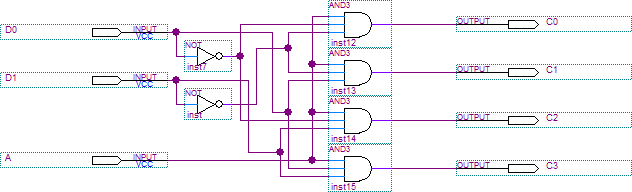
\includegraphics[width=\textwidth]{demultiplexer}
        \caption{Схема демультиплексора \( 2\times4 \)}
        \label{pic_dmx}
    \end{minipage}
    \hfill
    \begin{minipage}{.25\textwidth}
        \centering
        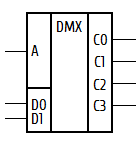
\includegraphics{dmx}
        \caption{Обозначение демультиплексоров на схемах}
        \label{pic_dmx_s}
    \end{minipage}
\end{figure}

На базе рассмотренных четырех устройств можно построить различные
комбинационные устройства с минимальным числом дополнительных элементов логики.

\newpage % --------------------------------------------------------------------
\renewcommand{\bibname}{Список источников}

\begin{thebibliography}{9} \addcontentsline{toc}{section}{Список источников}
    \bibitem{1} \href{http://ivatv.narod.ru/zifrovaja\_texnika/1\_05.htm}
    {http://ivatv.narod.ru/zifrovaja\_texnika/1\_05.htm}
    \bibitem{2} \href{http://life-prog.ru/view\_automati.php?id=14}
    {http://life-prog.ru/view\_automati.php?id=14}
    \bibitem{3} \href{http://roboforum.ru/wiki/Шифратор}
    {http://roboforum.ru/wiki/Шифратор}
    \bibitem{4} \href{http://roboforum.ru/wiki/Дешифратор}
    {http://roboforum.ru/wiki/Дешифратор}
    \bibitem{5} \href{http://http://ru.wikipedia.org/wiki/Шифратор\_(электроника)}
    {http://http://ru.wikipedia.org/wiki/Шифратор\_(электроника)}
    \bibitem{6} \href{http://http://ru.wikipedia.org/wiki/Дешифратор}
    {http://http://ru.wikipedia.org/wiki/Дешифратор}
    \bibitem{7} \href{http://marshal-group.com/shifrator-eto-kodoviy.html}
    {http://marshal-group.com/shifrator-eto-kodoviy.html}
\end{thebibliography}